\subsection*{Interpretability}
%--------------------------------------------------------------------------------------------------
\begin{frame}[c]
    \frametitle{Interpretability}
    \framesubtitle{Two dimension grouping}
    \pause
    \begin{columns}
        \column{0.5\textwidth}
        \textbf{Transparency}\\
        Approaches requiring changes to an architecture or training process.
        \column{0.5\textwidth}
        \textbf{Post-Hoc Interpretability}\\
        Approaches utilizing information contained within a model.
    \end{columns}
    
\end{frame}
%--------------------------------------------------------------------------------------------------
\begin{frame}[t]
    \frametitle{Interpretability}
    \framesubtitle{Class Activation Methods}
    Semantic information is found in deeper stages of a model \cite{lee2009convolutional}. \\
    \begin{center}
        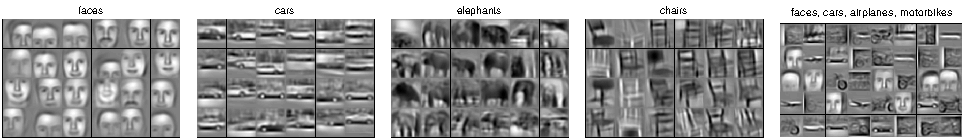
\includegraphics[width=\textwidth]{fig/rel/interp/img/conv_layers.pdf}
    \end{center}
    \pause
    Salient regions are highlighted for an input image:
    \begin{center}
        \resizebox{.8\textwidth}{!}{%}
         \begin{tikzpicture}[
    font={\footnotesize},
    trap/.style={trapezium, rotate=-90,trapezium angle=75},
]
    %% Nodes
    \node(input) at (-6, 0) {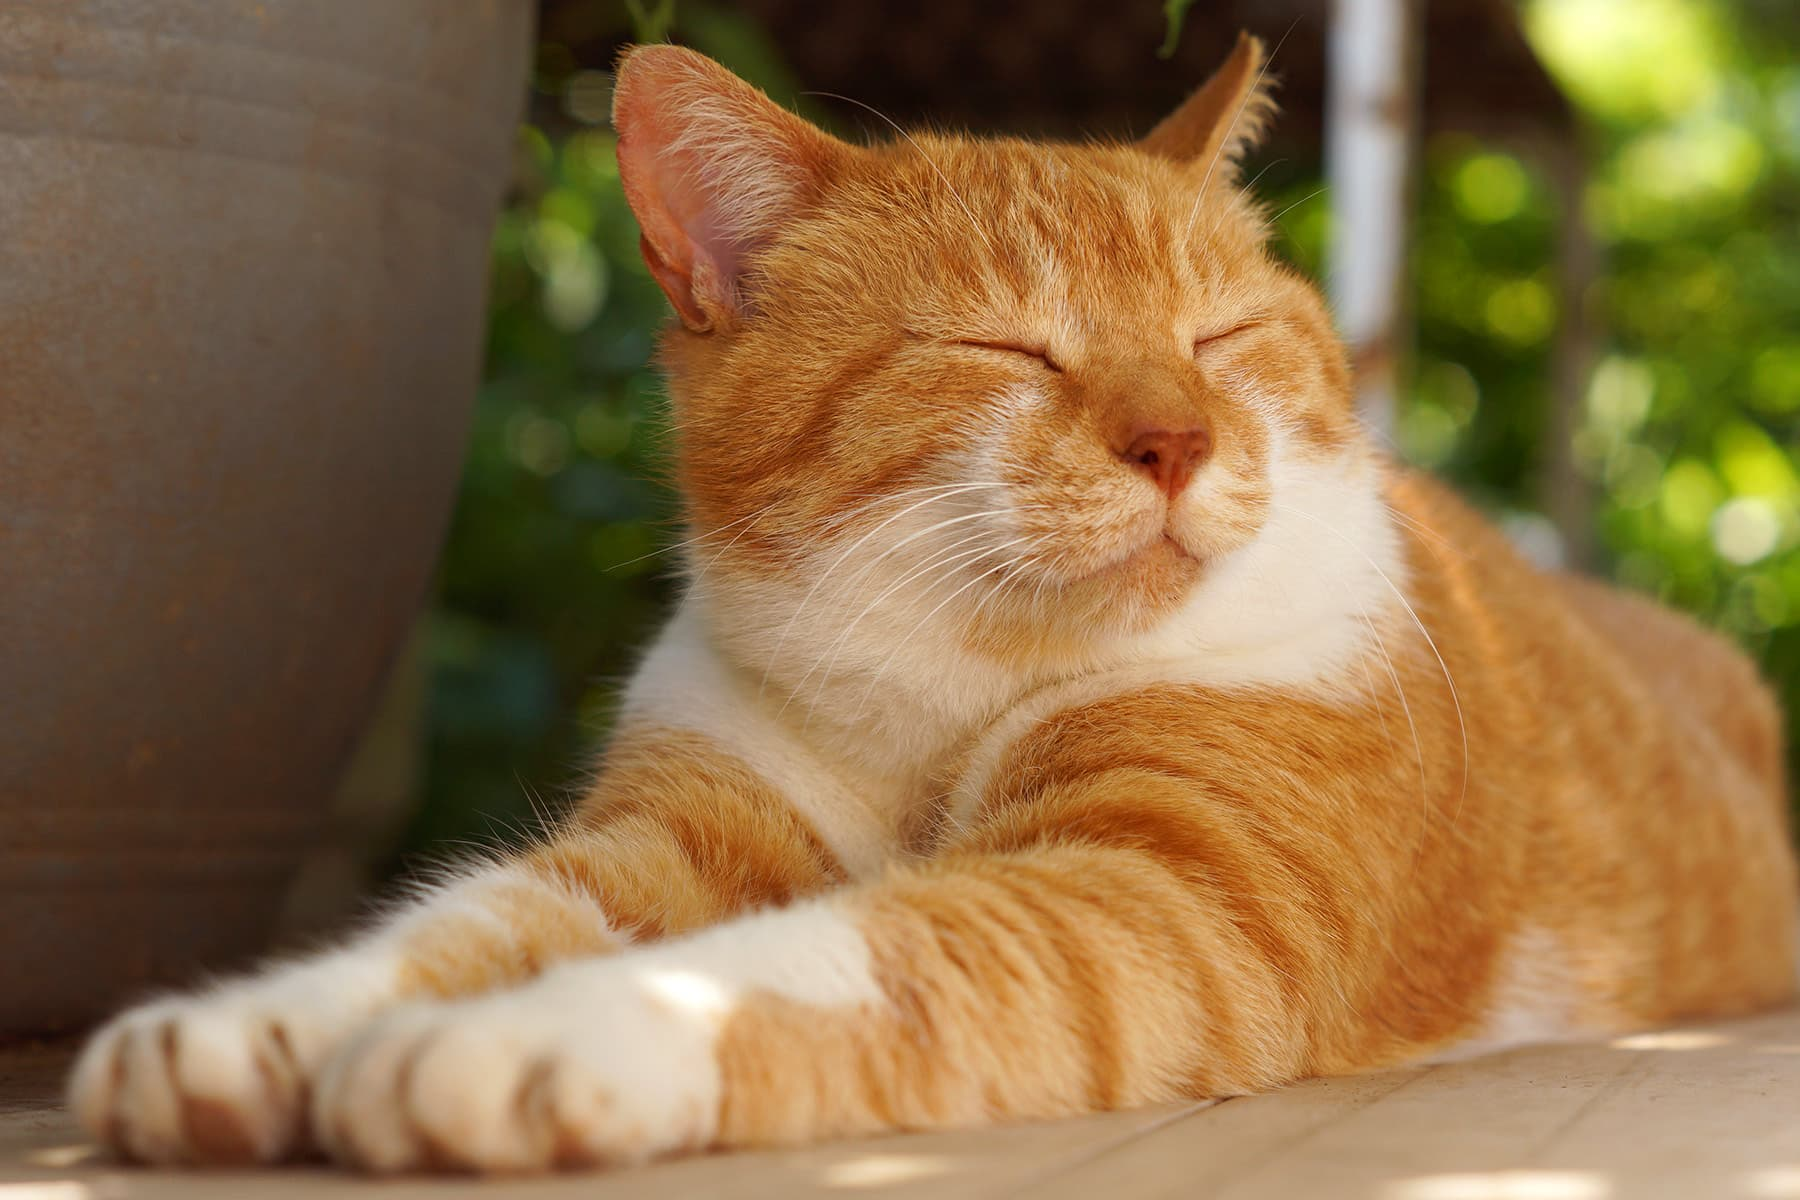
\includegraphics[width=.1\textwidth]{fig/rel/interp/img/cat_v2.jpg}};
    \node[above] at (input.north) {Input image $\vumod$};
    \node[draw, trap](cnn) at (-3, 0) {\rotatebox{90}{\parbox{1.0cm}{\centering{\Th{CNN}}}}};
    \node(fmaps) at (-0.5,0) {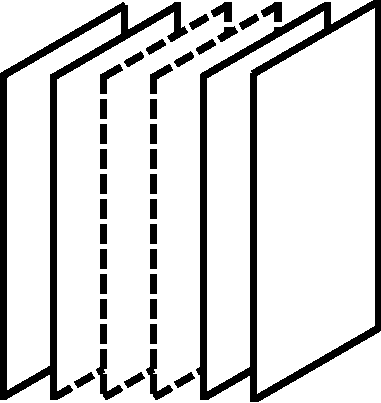
\includegraphics[width=.1\textwidth]{fig/rel/interp/img/fmaps_side.pdf}};
    \node(fmk) at (-0.5, 1.3) {$A^k_\ell$};
    \node(classtag) at (3, 1.3) {\Th{Classifier}};
    \node(GAP) at (1.25,0.25) {\Th{GAP}};
    \node(gapclass) at (3, 0) {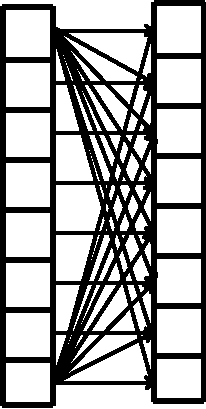
\includegraphics[width=.075\textwidth]{fig/rel/interp/img/gapclass.pdf}};
    \node(logit) at (5, 0) {$\vy_c$};
    \node(wck) at (-0.5, -3) {
\includegraphics[width=0.02\textwidth, angle=90]{fig/rel/interp/img/classifier.pdf}};
    \node(comb) at (-0.5, -3.5) {Weighting coefficient $w_k^c$};
    \node[draw, circle] (odot) at (-0.5, -1.8) {$\times$};
    \node(activ) at (-2.75, -1.5) {$h$};
    \node(salient) at (-3, -1.8) {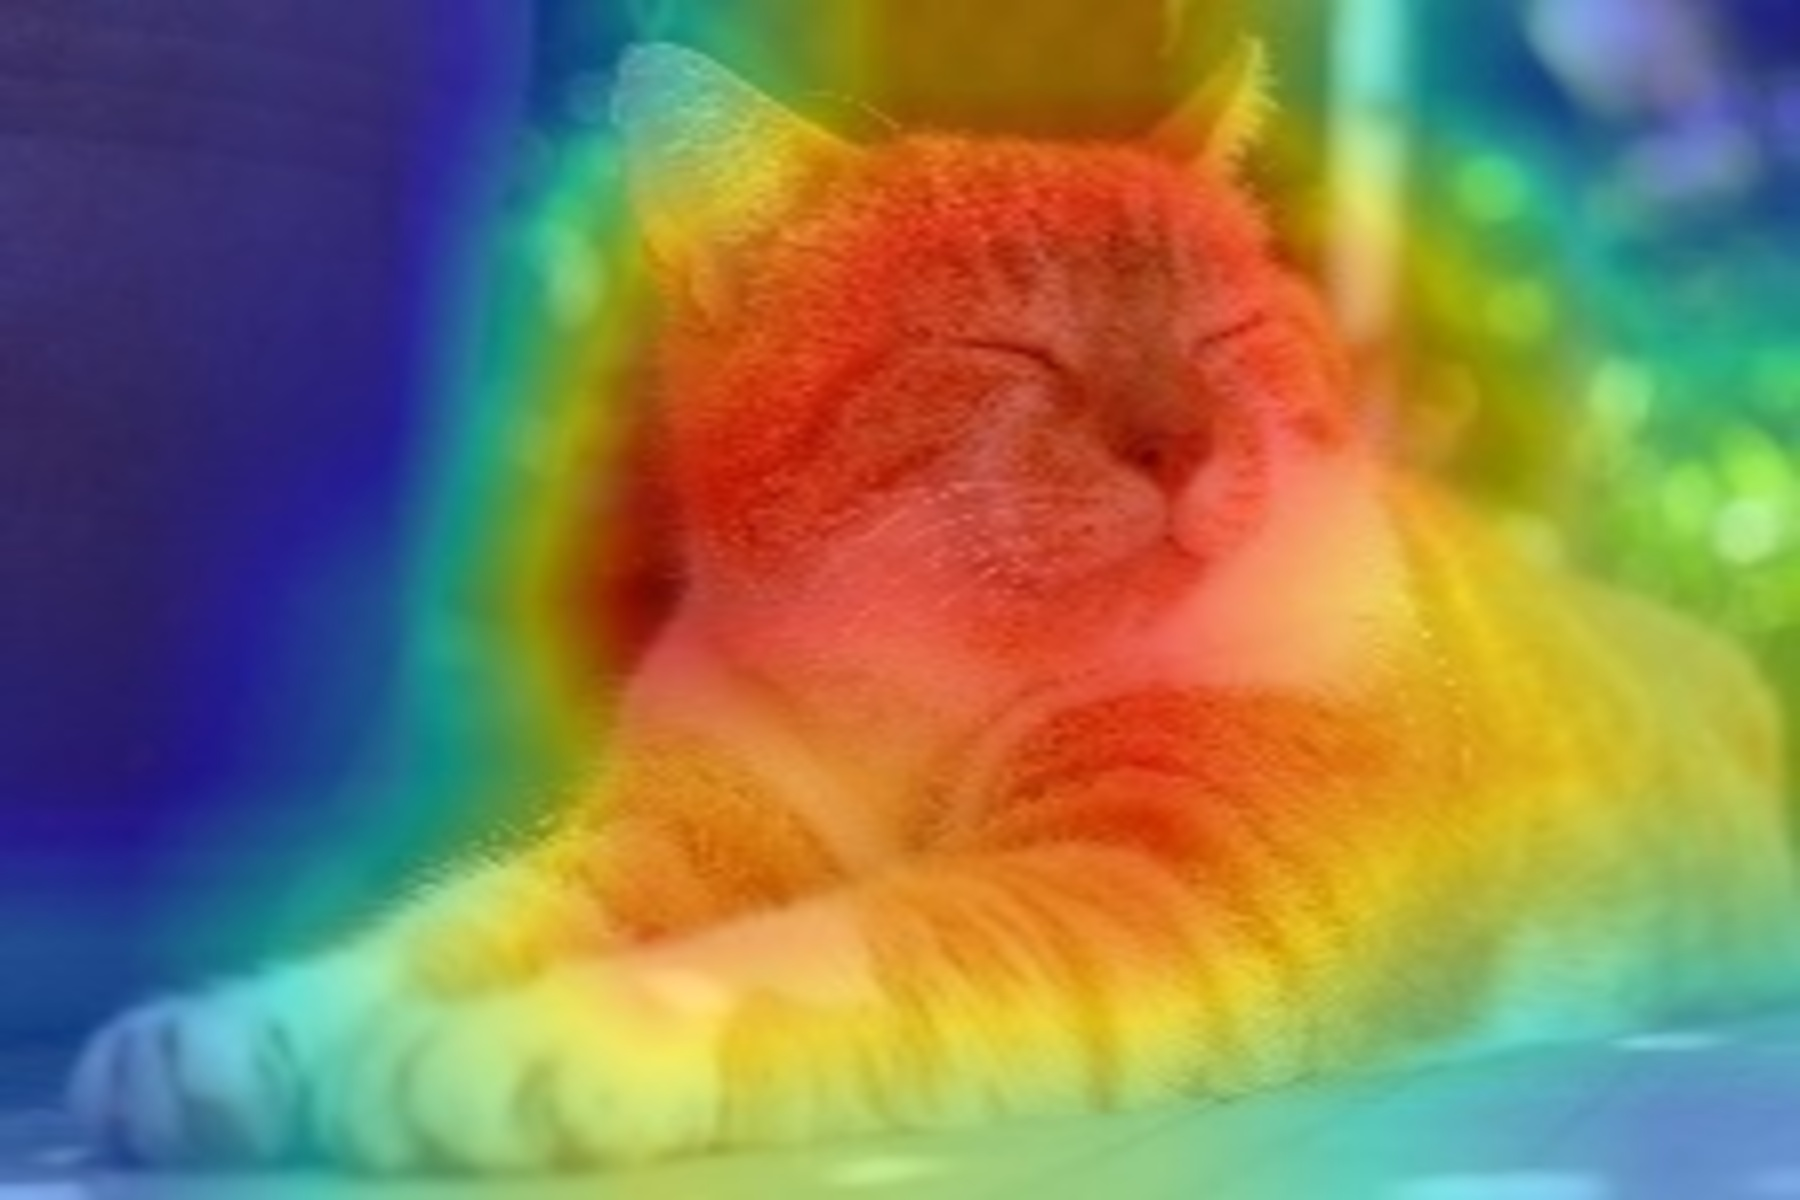
\includegraphics[width=.1\textwidth]{fig/rel/interp/img/cat_cam.jpg}};
    \node[below] at (salient.south) {Saliency map $\mathbf{S_\ell}$};
    \node[] at (4, -1.8) (eq_cam) {$S^c_\ell (\textbf{\mbox{u}}) \defn h \left(\sum_k w^c_k A^k_l \right)$};
    
    %% Edge
    \draw[->] (input.east) -- node {} (cnn);
    \draw[->] (cnn.north) -- node[above] {$\ell$} (fmaps.west);
    \draw[->] (fmaps.east) -- node {} (gapclass.west);
    \draw[->] (gapclass.east) -- node[above] {} (logit.west);
    \draw[->] (fmaps.south) -- node {} (odot.north);
    \draw[->] (wck.north) -- node {} (odot.south);
    \draw[->] (odot.west) -- node {} (salient);          
\end{tikzpicture}
         }
    \end{center}
\end{frame}
%--------------------------------------------------------------------------------------------------
\begin{frame}[t]
    \frametitle{Interpretability}
    \framesubtitle{Evaluating Interpretability}
    Saliency: what is relevant towards a prediction.\\
    An explanation should demonstrate similar predictive properties to its query.\\
    \vspace{20pt}
    \begin{columns}
        \column{0.3\textwidth}
            \begin{center}
                {\scriptsize Input image. ($I$)}\\
                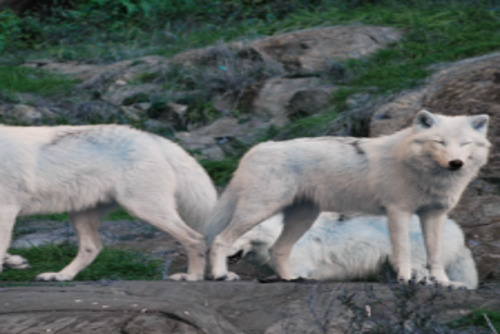
\includegraphics[width=\textwidth]{fig/rel/interp/img/ILSVRC2012_val_00000027.JPEG}\\
                {\scriptsize $Y^c_i = 0.8756$}
            \end{center}
        \column{0.3\textwidth}
            \begin{center}
                {\scriptsize Explanation Map. ($E^c$)}\\
                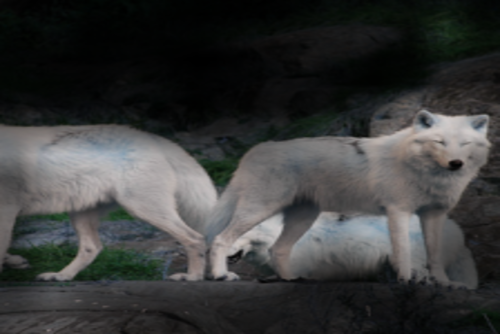
\includegraphics[width=\textwidth]{fig/rel/interp/img/masked_resized.png}\\
                {\scriptsize $O^c_i = 0.7442$}
            \end{center}
        \pause
        \column{.4\textwidth}
            {\scriptsize%
                \begin{itemize}
                    \item Prediction loss when using an explanation. (Average Drop 
                        (AD) \cite{chattopadhay2018grad})
                    \item Ratio of explanations being better than the input image. (Average Increase 
                        (AI) \cite{chattopadhay2018grad})
                    \item Reaction to saliency guided modifications (Insertion/Deletion 
                        (Ins/Del) \cite{petsiuk2018rise}) 
                \end{itemize}
            }
    \end{columns}
    
\end{frame}